\documentclass[oneside]{book}\usepackage[]{graphicx}\usepackage[svgnames]{xcolor}
% maxwidth is the original width if it is less than linewidth
% otherwise use linewidth (to make sure the graphics do not exceed the margin)
\makeatletter
\def\maxwidth{ %
  \ifdim\Gin@nat@width>\linewidth
    \linewidth
  \else
    \Gin@nat@width
  \fi
}
\makeatother

\definecolor{fgcolor}{rgb}{0.345, 0.345, 0.345}
\newcommand{\hlnum}[1]{\textcolor[rgb]{0.686,0.059,0.569}{#1}}%
\newcommand{\hlstr}[1]{\textcolor[rgb]{0.192,0.494,0.8}{#1}}%
\newcommand{\hlcom}[1]{\textcolor[rgb]{0.678,0.584,0.686}{\textit{#1}}}%
\newcommand{\hlopt}[1]{\textcolor[rgb]{0,0,0}{#1}}%
\newcommand{\hlstd}[1]{\textcolor[rgb]{0.345,0.345,0.345}{#1}}%
\newcommand{\hlkwa}[1]{\textcolor[rgb]{0.161,0.373,0.58}{\textbf{#1}}}%
\newcommand{\hlkwb}[1]{\textcolor[rgb]{0.69,0.353,0.396}{#1}}%
\newcommand{\hlkwc}[1]{\textcolor[rgb]{0.333,0.667,0.333}{#1}}%
\newcommand{\hlkwd}[1]{\textcolor[rgb]{0.737,0.353,0.396}{\textbf{#1}}}%
\let\hlipl\hlkwb

\usepackage{framed}
\makeatletter
\newenvironment{kframe}{%
 \def\at@end@of@kframe{}%
 \ifinner\ifhmode%
  \def\at@end@of@kframe{\end{minipage}}%
  \begin{minipage}{\columnwidth}%
 \fi\fi%
 \def\FrameCommand##1{\hskip\@totalleftmargin \hskip-\fboxsep
 \colorbox{shadecolor}{##1}\hskip-\fboxsep
     % There is no \\@totalrightmargin, so:
     \hskip-\linewidth \hskip-\@totalleftmargin \hskip\columnwidth}%
 \MakeFramed {\advance\hsize-\width
   \@totalleftmargin\z@ \linewidth\hsize
   \@setminipage}}%
 {\par\unskip\endMakeFramed%
 \at@end@of@kframe}
\makeatother

\definecolor{shadecolor}{rgb}{.97, .97, .97}
\definecolor{messagecolor}{rgb}{0, 0, 0}
\definecolor{warningcolor}{rgb}{1, 0, 1}
\definecolor{errorcolor}{rgb}{1, 0, 0}
\newenvironment{knitrout}{}{} % an empty environment to be redefined in TeX

\usepackage{alltt}
\usepackage[svgnames]{xcolor}
\usepackage[british]{babel}
\usepackage[protrusion,expansion,babel,final]{microtype}
\usepackage[margin=1in]{geometry}
\usepackage[pdfversion=1.7]{hyperref}
\usepackage[shortlabels]{enumitem}
\usepackage{graphicx}
\usepackage{mathtools}
\usepackage{cleveref}
\usepackage{booktabs}
\usepackage{nicematrix}
\usepackage{derivative}
\usepackage{etoolbox}
\usepackage{siunitx}
\usepackage{lmodern}
\usepackage[T1]{fontenc}
\usepackage[scaled=.98]{XCharter}
\usepackage[scaled=1.04,varqu,varl]{inconsolata}% inconsolata typewriter
\usepackage{amssymb}
\makeatletter
\@namedef{T1/zi4/m/it}{<->ssub*lmr/m/it}
\makeatother

\usepackage{bm}
\usepackage{tikz}
\usepackage{float}

% Functions
\providecommand\given{} % just to make sure it exists
\DeclarePairedDelimiterXPP{\E}[1]{\operatorname{\mathbb{E}}}[]{}{%
    \renewcommand\given{\nonscript\:\delimsize\vert\nonscript\:\mathopen{}}%
    \ifblank{#1}{\:\cdot\:}%
    #1}%
\DeclarePairedDelimiterXPP{\V}[1]{\operatorname{\textsf{V}}}(){}{%
    \renewcommand\given{\nonscript\:\delimsize\vert\nonscript\:\mathopen{}}%
    \ifblank{#1}{\:\cdot\:}%
    #1}%
\DeclarePairedDelimiterXPP{\Var}[1]{\operatorname{\textsf{Var}}}(){}{%
    \renewcommand\given{\nonscript\:\delimsize\vert\nonscript\:\mathopen{}}%
    \ifblank{#1}{\:\cdot\:}%
    #1}%
\DeclarePairedDelimiterXPP{\Cov}[1]{\operatorname{\textsf{Cov}}}(){}{%
    \renewcommand\given{\nonscript\:\delimsize\vert\nonscript\:\mathopen{}}%
    \ifblank{#1}{\:\cdot\:}%
    #1}%
\DeclarePairedDelimiterXPP{\Corr}[1]{\operatorname{\textsf{Corr}}}(){}{%
    \renewcommand\given{\nonscript\:\delimsize\vert\nonscript\:\mathopen{}}%
    \ifblank{#1}{\:\cdot\:}%
    #1}%
\DeclarePairedDelimiterXPP{\Covadj}[1]{\operatorname{\textsf{Cov}_{\text{adj}}}}(){}{%
    \renewcommand\given{\nonscript\:\delimsize\vert\nonscript\:\mathopen{}}%
    \ifblank{#1}{\:\cdot\:}%
    #1}%
\DeclarePairedDelimiterXPP\Prob[1]{\operatorname{\mathbb{P}}}(){}{%
    \renewcommand\given{\nonscript\:\delimsize\vert\nonscript\:\mathopen{}}%
    \ifblank{#1}{\:\cdot\:}%
    #1}%
\DeclarePairedDelimiterXPP\Ind[1]{\operatorname{\mathbb{I}}}\{\}{}{%
    \renewcommand\given{\nonscript\:\delimsize\vert\nonscript\:\mathopen{}}%
    \ifblank{#1}{\:\cdot\:}%
    #1}%
\DeclarePairedDelimiterXPP{\se}[1]{\operatorname{\textsf{se}}}(){}{%
    \ifblank{#1}{\:\cdot\:}%
    #1}%
\DeclarePairedDelimiterXPP{\seadj}[1]{\operatorname{\textsf{se}_{\text{adj}}}}(){}{%
    \renewcommand\given{\nonscript\:\delimsize\vert\nonscript\:\mathopen{}}%
    \ifblank{#1}{\:\cdot\:}%
    #1}%
\DeclarePairedDelimiterXPP{\estseadj}[1]{\operatorname{\widehat{\textsf{se}}_{\text{adj}}}}(){}{%
    \renewcommand\given{\nonscript\:\delimsize\vert\nonscript\:\mathopen{}}%
    \ifblank{#1}{\:\cdot\:}%
    #1}%
\DeclarePairedDelimiterXPP{\estse}[1]{\widehat{\operatorname{\textsf{se}}}}(){}{%
    \ifblank{#1}{\:\cdot\:}%
    #1}%
\DeclarePairedDelimiterXPP{\estV}[1]{\widehat{\operatorname{\textsf{V}}}}(){}{
    \renewcommand\given{\nonscript\:\delimsize\vert\nonscript\:\mathopen{}}%
    \ifblank{#1}{\:\cdot\:}%
    #1}%
\DeclarePairedDelimiterXPP{\estVar}[1]{\widehat{\operatorname{\textsf{Var}}}}(){}{
    \renewcommand\given{\nonscript\:\delimsize\vert\nonscript\:\mathopen{}}%
    \ifblank{#1}{\:\cdot\:}%
    #1}%
\let\exp\relax%
\let\log\relax%
\let\ln\relax%
\DeclarePairedDelimiterXPP{\exp}[1]{\operatorname{\textsf{exp}}}\{\}{}{#1}%
\DeclarePairedDelimiterXPP{\log}[1]{\operatorname{\textsf{log}}}(){}{#1}%
\DeclarePairedDelimiterXPP{\ln}[1]{\operatorname{\textsf{ln}}}(){}{#1}%
\DeclarePairedDelimiterXPP{\diag}[1]{\operatorname{\textsf{diag}}}(){}{#1}%
\DeclarePairedDelimiterXPP{\sign}[1]{\operatorname{\textsf{sign}}}(){}{#1}%

\DeclarePairedDelimiterXPP{\expit}[1]{\operatorname{\textsf{expit}}}(){}{#1}%
\DeclarePairedDelimiterXPP{\logit}[1]{\operatorname{\textsf{logit}}}(){}{#1}%
\newcommand{\HN}{\textsl{H}_{\textsl{0}}}%
\newcommand{\HA}{\textsl{H}_{\textsl{A}}}%

% Distributions
\DeclarePairedDelimiterXPP{\N}[1]{\mathcal{N}}(){}{#1}%
\DeclarePairedDelimiterXPP{\POI}[1]{\text{POI}}(){}{#1}%
\DeclarePairedDelimiterXPP{\BIN}[1]{\text{BIN}}(){}{#1}%
\DeclarePairedDelimiterXPP{\BERN}[1]{\text{BERN}}(){}{#1}%
\DeclarePairedDelimiterXPP{\MVN}[1]{\text{MVN}}(){}{#1}%
\DeclarePairedDelimiterXPP{\NB}[1]{\text{NB}}(){}{#1}%
\DeclarePairedDelimiterXPP{\GAM}[1]{\text{GAM}}(){}{#1}%
\DeclarePairedDelimiterXPP{\BetaDist}[1]{\text{Beta}}(){}{#1}%

\newcommand{\iid}{\overset{\text{iid}}{\sim}}%
\newcommand{\ind}{\overset{\text{ind}}{\sim}}%
\newcommand{\OR}{\text{OR}}%
\newcommand{\RR}{\text{RR}}%
\newcommand{\cOR}{\text{cOR}}%

\DeclarePairedDelimiter\abs{\lvert}{\rvert}
% can be useful to refer to this outside \Set
\newcommand\SetSymbol[1][]{%
    \nonscript\:#1\vert{}
    \allowbreak\nonscript\:
    \mathopen{}}
\DeclarePairedDelimiterX\Set[1]\{\}{%
    \renewcommand\given{:}
    #1
}
\DeclareMathOperator*{\argmax}{arg\,max}
\DeclareMathOperator*{\argmin}{arg\,min}
\DeclareMathOperator*{\arginf}{arg\,inf}
\DeclareMathOperator*{\argsup}{arg\,sup}

\providecommand{\RandomVector}[1]{\bm{#1}}% general vectors in bold italic
\providecommand{\Vector}[1]{\bm{#1}}% general vectors in bold italic
\providecommand{\Matrix}[1]{\bm{#1}}
\providecommand{\MatrixCal}[1]{\bm{\mathcal{#1}}}
\providecommand{\Field}[1]{\bm{#1}}

\usepackage{stackengine}
\usepackage[british]{isodate}
\newcommand{\makeheading}[2]%
{%
\begin{center}%
    \makebox[\linewidth]{\raisebox{-.5ex}[0cm][0cm]{\stackanchor{\textcolor{Gray}{\textsc{#1}}}{\scriptsize\itshape\printyearoff#2}\;}\color{Crimson!50}\hrulefill}%
\end{center}%
}%

\usepackage[breakable]{tcolorbox}
\tcbset{
    regular/.style={
        boxrule=0pt,
        breakable,
        sharp corners
    }
}

\newtcolorbox{Example}[1]{regular,colframe=Green!20!white,colback=Green!10!white,coltitle=Green,title={#1}}%
\newtcolorbox{Regular}[1]{regular,colframe=Navy!15!white,colback=Navy!5!white,coltitle=Navy,title={#1}}%
\newtcolorbox{Result}[1]{regular,colframe=Red!15!white,colback=Red!5!white,coltitle=Red,title={#1}}%

\hypersetup{colorlinks=true,%
linkcolor=[rgb]{0,0.5,1},%
pdftitle={Statistical Methods for Life History Analysis (STAT 437)},%
pdfauthor={Cameron Roopnarine, Dylan Spicker},%
pdfsubject={Statistics},%
pdfkeywords={University of Waterloo, Winter 2022 (1221)}}%

\title{%
\LARGE Statistical Methods for Life History Analysis\\%
\large STAT 437\\%
\normalsize Winter 2022 (1221)\thanks{Online Course}}%
\author{Cameron Roopnarine\thanks{\LaTeX{}er}\and Dylan Spicker\thanks{Instructor}}%
\date{\today}%
\usepackage{pgfplots}
\pgfplotsset{compat=1.18}
\usetikzlibrary{petri,decorations.pathreplacing,calc}
\IfFileExists{upquote.sty}{\usepackage{upquote}}{}
\begin{document}


\maketitle
\tableofcontents
\chapter{What are Longitudinal Data?}
\makeheading{Week 1}{\daterange{2022-01-05}{2022-01-07}}%chktex 8
\section{What are Longitudinal Data?}
\begin{figure}[H]
    \centering
    
\includegraphics[width=\textwidth]{figures/002-study.pdf}
\end{figure}
What would a study \textbf{need} to look like to conclude this?
\subsection{The Design of a Longitudinal Study}
\begin{itemize}
    \item Can we conclude this by taking a sample of elderly individuals directly?
          \begin{itemize}
              \item \textbf{No}. How do we determine how much they slept 20 years prior?
          \end{itemize}
    \item Can we conclude this by taking a sample of middle-aged individuals directly?
          \begin{itemize}
              \item \textbf{No}. How do we determine who will develop dementia later on?
          \end{itemize}
    \item Can we conclude this by taking independent samples of middle-aged individuals \emph{and}
          elderly individuals?
          \begin{itemize}
              \item \textbf{No}. How do we pair the individuals?
          \end{itemize}
\end{itemize}
We would \emph{need} to be able to follow individuals, starting when they are middle-aged,
recording information like how often they sleep, and continue following them until the
onset of dementia.
\begin{framed}
    \centering\textbf{This is a longitudinal study}.
\end{framed}
\begin{figure}[H]
    \centering
    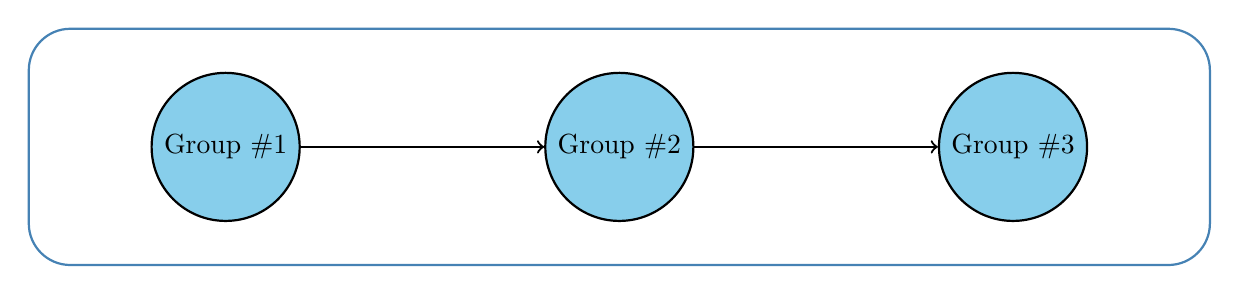
\begin{tikzpicture}[thick]
        \draw[rounded corners=15pt,SteelBlue] (10,0) rectangle ++(15,3);
        \node[draw,circle,fill=SkyBlue] (A) at (12.5,1.5) {Group \#1};
        \node[draw,circle,fill=SkyBlue] (B) at (17.5,1.5) {Group \#2};
        \node[draw,circle,fill=SkyBlue] (C) at (22.5,1.5) {Group \#3};
        \draw[->] (A) -- (B);
        \draw[->] (B) -- (C);
    \end{tikzpicture}
    \caption{Longitudinal Study}
\end{figure}
\begin{figure}[H]
    \centering
    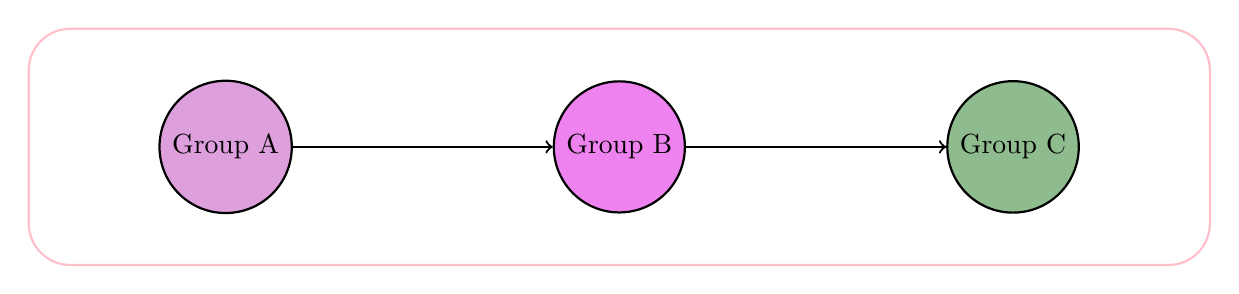
\begin{tikzpicture}[thick]
        \draw[rounded corners=15pt,Pink] (10,0) rectangle ++(15,3);
        \node[draw,circle,fill=Plum] (A) at (12.5,1.5) {Group A};
        \node[draw,circle,fill=Violet] (B) at (17.5,1.5) {Group B};
        \node[draw,circle,fill=DarkSeaGreen] (C) at (22.5,1.5) {Group C};
        \draw[->] (A) -- (B);
        \draw[->] (B) -- (C);
    \end{tikzpicture}
    \caption{Cross-Sectional Study}
\end{figure}
A research study in which \textbf{subjects are followed over time}.
Typically, this involves
repeated measurements of the same variables.
Longitudinal studies differ from \textbf{cross-sectional} studies and
\textbf{time series} studies.
\subsection{Uses for Longitudinal Studies}
\begin{itemize}
    \item To detect \emph{changes} in outcomes, both at the population and individual level.
    \item \textbf{Longitudinal effects} as compared to \textbf{cohort effects}.
    \item Correctly ascertain the exposures.
    \item Understand different sources of variation
    \item \textbf{Between}- and \textbf{within}-subject variation.
    \item To detect \textbf{time effects}, both directly and as interactions with other relevant
          factors.
\end{itemize}
Bottom line: There are many questions of interest which can only be answered using
longitudinal data. We should probably learn how to analyse it.
\subsection{Why are Longitudinal Data Special?}
What makes longitudinal data more difficult to analyse?
\begin{itemize}
    \item The data are \textbf{correlated}.
    \item Everyone's favourite assumption
          (assume that $ X_1,\ldots,X_n $ are iid) will \textbf{not} hold.
    \item Now what? STAT 437.
\end{itemize}
\subsection{Example Datasets}
\subsubsection{TLC Trial}
\begin{table}[H]
    \centering
    \begin{tabular}{cccccc}
        \toprule
        ID     & Treatment & W0     & W1     & W4     & W6     \\
        \midrule
        1      & P         & 30.8   & 26.9   & 25.8   & 23.8   \\
        2      & A         & 26.5   & 14.8   & 19.5   & 21     \\
        3      & A         & 25.8   & 23     & 19.1   & 23.2   \\
        \vdots & \vdots    & \vdots & \vdots & \vdots & \vdots \\
        98     & A         & 29.4   & 22.1   & 25.3   & 4.1    \\
        99     & A         & 21.9   & 7.6    & 10.8   & 13     \\
        100    & A         & 20.7   & 8.1    & 25.7   & 12.3   \\
        \bottomrule
    \end{tabular}
\end{table}
\begin{itemize}
    \item Is there a difference between \textbf{placebo} and \textbf{treatment}?
    \item How does the blood lead level \textbf{change over time} (in each group)?
    \item Is the \textbf{change} over time \textbf{equal} between treatment groups?
\end{itemize}
\subsubsection{Sales Data}
\begin{table}[H]
    \centering
    \begin{tabular}{ccccc}
        \toprule
        \texttt{DATE} & \texttt{brand} & \texttt{prod} & \texttt{QTY} & \texttt{PROMO} \\
        \midrule
        2014-01-02    & 1              & 1             & 7            & 0              \\%chktex 8
        2014-01-02    & 1              & 2             & 3            & 0              \\%chktex 8
        2014-01-02    & 1              & 3             & 0            & 0              \\%chktex 8
        \vdots        & \vdots         & \vdots        & \vdots       & \vdots         \\%chktex 8
        2018-12-31    & 4              & 8             & 1            & 1              \\%chktex 8
        2018-12-31    & 4              & 9             & 0            & 0              \\%chktex 8
        2018-12-31    & 4              & 10            & 3            & 1              \\%chktex 8
        \bottomrule
    \end{tabular}
\end{table}
\begin{itemize}
    \item Are the \textbf{different brands comparable} in terms of overall sales?
    \item Are the \textbf{different products comparable}?
    \item Do \textbf{promotions increase} the quantity sold? If so, \textbf{by how much}?
    \item Do the effects of time, and promotion, \textbf{change by brand} or product?
\end{itemize}
\subsubsection{Podcast Data}
\begin{table}[H]
    \centering
    \begin{tabular}{ccccc}
        \toprule
        Rating & No. Reviews & Title                  & Date       & $\cdots$ \\
        \midrule
        4.9    & 6400        & Dissect                & 2019-11-01 & $\cdots$ \\%chktex 8
        4.9    & 26300       & The Adventure Zone     & 2019-11-01 & $\cdots$ \\%chktex 8
        4.8    & 3700        & Song Exploder          & 2019-11-01 & $\cdots$ \\%chktex 8
        \vdots & \vdots      & \vdots                 & \vdots     & \vdots   \\%chktex 8
        4.2    & 1100        & Finding Fred           & 2019-12-01 & $\cdots$ \\%chktex 8
        3.9    & 648         & Inside Frozen 2        & 2019-12-01 & $\cdots$ \\%chktex 8
        4.6    & 6400        & Pop Culture Happy Hour & 2019-12-01 & $\cdots$ \\%chktex 8
        \bottomrule
    \end{tabular}
\end{table}
\begin{itemize}
    \item Can we \textbf{predict} the number of ratings that a podcast will receive over time?
    \item Can we \textbf{predict} the average rating value that a podcast will receive over time?
\end{itemize}
\subsubsection{Stroke Data}
\[ \begin{array}{ccccc}
        \toprule
        \texttt{year} & \text{Prop.}~(0,0) & \text{Prop.}~(0,1) & \text{Prop.}~(1,0) & \text{Prop.}~(1,1) \\
        \midrule
        1             & 57 / 344           & 17 / 72            & 17 / 79            & 5 / 23             \\
        2             & 27 / 287           & 8 / 55             & 9 / 62             & 4 / 18             \\
        3             & 23 / 260           & 8 / 47             & 5 / 53             & 3 / 14             \\
        \vdots        & \vdots             & \vdots             & \vdots             & \vdots             \\
        8             & 10 / 129           & 1 / 15             & 5 / 23             & 1 / 4              \\
        9             & 17 / 119           & 3 / 14             & 4 / 18             & 0 / 3              \\
        10            & 13 / 102           & 1 / 11             & 2 / 14             & 0 / 3              \\
        \bottomrule
    \end{array} \]
\begin{itemize}
    \item $0 =$ placebo treatment, $1 =$ active treatment; $0 =$ no previous stroke, $1 =$ previous stroke.
    \item This is \textbf{time to event} data.
    \item What is \textbf{probability of surviving} beyond some point?
    \item Does this \textbf{differ} if you previously had a stroke? If you \textbf{received treatment}?
\end{itemize}
\subsection{Summary}
\begin{itemize}
    \item Longitudinal data occur when we take repeated measurements on the same
          individuals over time.
    \item Longitudinal data are required for answering questions about changes within an
          individual (compared to between individuals) and to capture time effects.
    \item Longitudinal data are challenging to work with because the data are correlated.
\end{itemize}

\section{Exploring Longitudinal Data (Application)}
%\begin{noindent}
\begin{knitrout}
\definecolor{shadecolor}{rgb}{0.969, 0.969, 0.969}\color{fgcolor}\begin{kframe}
\begin{alltt}
\hlcom{# Read in the TLC Data Note: This is stored for me at}
\hlcom{# data/TLC/TLC.csv, you should update for yourself}
\hlstd{TLC} \hlkwb{<-} \hlkwd{read.csv}\hlstd{(}\hlstr{"data/TLC/TLC.csv"}\hlstd{)}
\hlkwd{head}\hlstd{(TLC)}  \hlcom{# Outputs the first few rows of the data to take a look}
\end{alltt}
\begin{verbatim}
  ID Treatment   W0   W1   W4   W6
1  1         P 30.8 26.9 25.8 23.8
2  2         A 26.5 14.8 19.5 21.0
3  3         A 25.8 23.0 19.1 23.2
4  4         P 24.7 24.5 22.0 22.5
5  5         A 20.4  2.8  3.2  9.4
6  6         A 20.4  5.4  4.5 11.9
\end{verbatim}
\begin{alltt}
\hlcom{# Convert from 'wide' to 'long' and back again, using}
\hlcom{# reshape.  If you're interested, you can also use}
\hlcom{# `pivot_wider` and `pivot_longer` from the tidyverse (If}
\hlcom{# that doesn't mean anything to you, feel free to ignore}
\hlcom{# it!)}
\hlstd{TLC_long} \hlkwb{<-} \hlkwd{reshape}\hlstd{(}\hlkwc{data} \hlstd{= TLC,} \hlkwc{varying} \hlstd{=} \hlkwd{c}\hlstd{(}\hlstr{"W0"}\hlstd{,} \hlstr{"W1"}\hlstd{,} \hlstr{"W4"}\hlstd{,}
  \hlstr{"W6"}\hlstd{),} \hlkwc{timevar} \hlstd{=} \hlstr{"week"}\hlstd{,} \hlkwc{idvar} \hlstd{=} \hlstr{"ID"}\hlstd{,} \hlkwc{times} \hlstd{=} \hlkwd{c}\hlstd{(}\hlnum{0}\hlstd{,} \hlnum{1}\hlstd{,} \hlnum{4}\hlstd{,}
  \hlnum{6}\hlstd{),} \hlkwc{direction} \hlstd{=} \hlstr{"long"}\hlstd{,} \hlkwc{sep} \hlstd{=} \hlstr{""}\hlstd{)}
\hlstd{TLC_wide} \hlkwb{<-} \hlkwd{reshape}\hlstd{(}\hlkwc{data} \hlstd{= TLC_long,} \hlkwc{timevar} \hlstd{=} \hlstr{"week"}\hlstd{,} \hlkwc{v.names} \hlstd{=} \hlstr{"W"}\hlstd{,}
  \hlkwc{idvar} \hlstd{=} \hlstr{"ID"}\hlstd{,} \hlkwc{times} \hlstd{=} \hlkwd{c}\hlstd{(}\hlnum{0}\hlstd{,} \hlnum{1}\hlstd{,} \hlnum{4}\hlstd{,} \hlnum{6}\hlstd{),} \hlkwc{direction} \hlstd{=} \hlstr{"wide"}\hlstd{,}
  \hlkwc{sep} \hlstd{=} \hlstr{""}\hlstd{)}
\hlcom{# Create a Basic Boxplot to get a Sense of the Data}
\hlkwd{boxplot}\hlstd{(W} \hlopt{~} \hlstd{week} \hlopt{+} \hlstd{Treatment,} \hlkwc{data} \hlstd{= TLC_long)}
\hlkwd{abline}\hlstd{(}\hlkwc{v} \hlstd{=} \hlnum{4.5}\hlstd{)}  \hlcom{# Abline v=... draws a vertical line at 4.5 }
\hlcom{# Start with an xyplot This requires the package 'lattice'}
\hlcom{# You can install using: install.packages('lattice')}
\hlstd{lattice}\hlopt{::}\hlkwd{xyplot}\hlstd{(W} \hlopt{~} \hlstd{week} \hlopt{|} \hlstd{Treatment,} \hlkwc{data} \hlstd{= TLC_long,} \hlkwc{groups} \hlstd{= ID,}
  \hlkwc{col} \hlstd{=} \hlstr{"black"}\hlstd{,} \hlkwc{type} \hlstd{=} \hlkwd{c}\hlstd{(}\hlstr{"l"}\hlstd{,} \hlstr{"p"}\hlstd{))}
\end{alltt}
\end{kframe}

{\centering 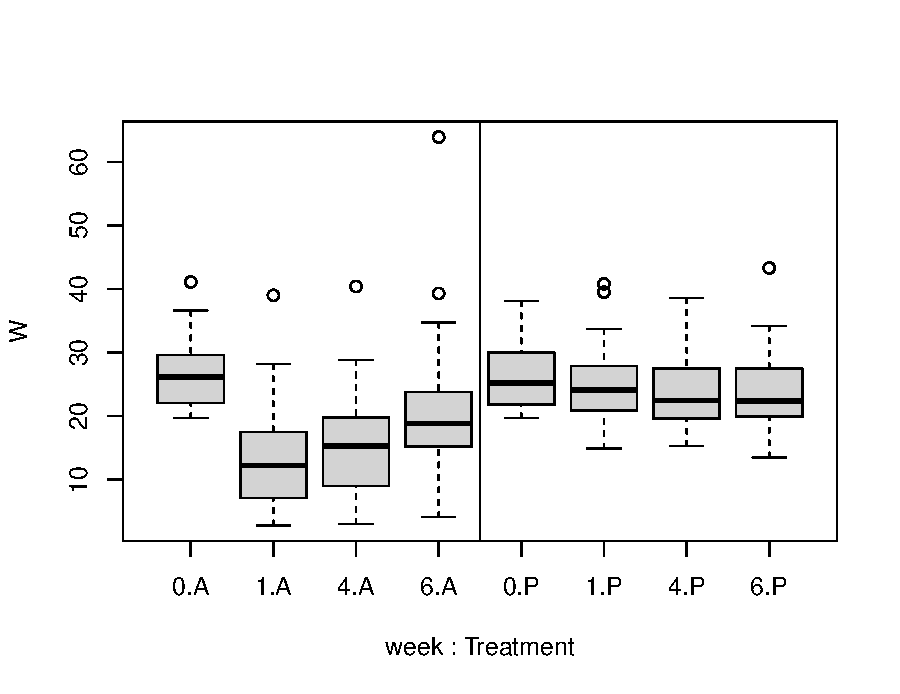
\includegraphics[width=\maxwidth]{figure/unnamed-chunk-3-1} 

}




{\centering 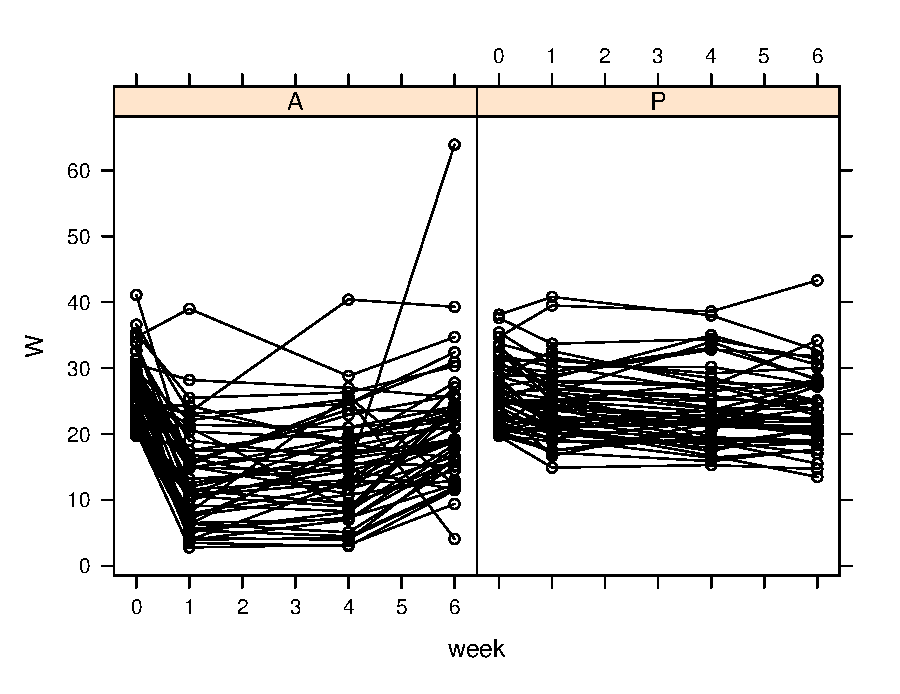
\includegraphics[width=\maxwidth]{figure/unnamed-chunk-3-2} 

}


\begin{kframe}\begin{alltt}
\hlcom{# The plot is a mess, as-is, so instead we can subset!}
\hlstd{plot_num} \hlkwb{<-} \hlnum{5}  \hlcom{# Select a fixed number}
\hlcom{# This is Just Randomly Sampling from Each Group}
\hlstd{random_samples_P} \hlkwb{<-} \hlkwd{sample}\hlstd{(}\hlkwd{unique}\hlstd{(TLC_long}\hlopt{$}\hlstd{ID[}\hlkwd{which}\hlstd{(TLC_long}\hlopt{$}\hlstd{Treatment} \hlopt{==}
  \hlstr{"P"}\hlstd{)]),} \hlkwc{size} \hlstd{= plot_num,} \hlkwc{replace} \hlstd{=} \hlnum{FALSE}\hlstd{)}
\hlstd{random_samples_A} \hlkwb{<-} \hlkwd{sample}\hlstd{(}\hlkwd{unique}\hlstd{(TLC_long}\hlopt{$}\hlstd{ID[}\hlkwd{which}\hlstd{(TLC_long}\hlopt{$}\hlstd{Treatment} \hlopt{==}
  \hlstr{"A"}\hlstd{)]),} \hlkwc{size} \hlstd{= plot_num,} \hlkwc{replace} \hlstd{=} \hlnum{FALSE}\hlstd{)}
\hlcom{## Actually Draw the Plots}
\hlkwd{par}\hlstd{(}\hlkwc{mfrow} \hlstd{=} \hlkwd{c}\hlstd{(}\hlnum{1}\hlstd{,} \hlnum{2}\hlstd{))}
\hlkwd{plot}\hlstd{(W} \hlopt{~} \hlstd{week,} \hlkwc{data} \hlstd{= TLC_long,} \hlkwc{subset} \hlstd{= (Treatment} \hlopt{==} \hlstr{"P"}\hlstd{))}
\hlkwa{for} \hlstd{(rid} \hlkwa{in} \hlstd{random_samples_P) \{}
  \hlcom{# Loop through the Random Points and Draw the}
  \hlcom{# Corresponding Lines}
  \hlkwd{lines}\hlstd{(W} \hlopt{~} \hlstd{week,} \hlkwc{data} \hlstd{= TLC_long,} \hlkwc{subset} \hlstd{= (ID} \hlopt{==} \hlstd{rid),} \hlkwc{type} \hlstd{=} \hlstr{"l"}\hlstd{)}
\hlstd{\}}
\hlcom{# Repeat it for Active Treatment}
\hlkwd{plot}\hlstd{(W} \hlopt{~} \hlstd{week,} \hlkwc{data} \hlstd{= TLC_long,} \hlkwc{subset} \hlstd{= (Treatment} \hlopt{==} \hlstr{"A"}\hlstd{))}
\hlkwa{for} \hlstd{(rid} \hlkwa{in} \hlstd{random_samples_A) \{}
  \hlkwd{lines}\hlstd{(W} \hlopt{~} \hlstd{week,} \hlkwc{data} \hlstd{= TLC_long,} \hlkwc{subset} \hlstd{= (ID} \hlopt{==} \hlstd{rid),} \hlkwc{type} \hlstd{=} \hlstr{"l"}\hlstd{)}
\hlstd{\}}
\end{alltt}
\end{kframe}

{\centering 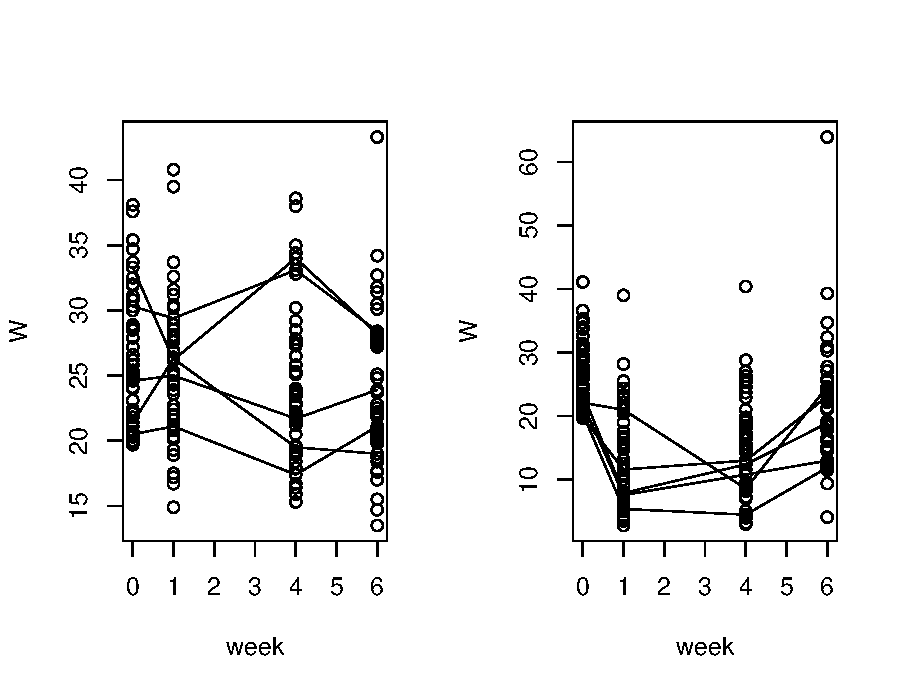
\includegraphics[width=\maxwidth]{figure/unnamed-chunk-3-3} 

}


\begin{kframe}\begin{alltt}
\hlcom{### Is there Smarter way of plotting?  What if we ordered}
\hlcom{### by the median observation?}
\hlstd{TLC_wide}\hlopt{$}\hlstd{median} \hlkwb{<-} \hlkwd{apply}\hlstd{(TLC_wide[}\hlkwd{c}\hlstd{(}\hlstr{"W0"}\hlstd{,} \hlstr{"W1"}\hlstd{,} \hlstr{"W4"}\hlstd{,} \hlstr{"W6"}\hlstd{)],}
  \hlkwc{MARGIN} \hlstd{=} \hlnum{1}\hlstd{,} \hlkwc{FUN} \hlstd{= median)}  \hlcom{# Generate the Medians}
\hlstd{TLC_long} \hlkwb{<-} \hlkwd{reshape}\hlstd{(}\hlkwc{data} \hlstd{= TLC_wide,} \hlkwc{varying} \hlstd{=} \hlkwd{c}\hlstd{(}\hlstr{"W0"}\hlstd{,} \hlstr{"W1"}\hlstd{,}
  \hlstr{"W4"}\hlstd{,} \hlstr{"W6"}\hlstd{),} \hlkwc{timevar} \hlstd{=} \hlstr{"week"}\hlstd{,} \hlkwc{idvar} \hlstd{=} \hlstr{"ID"}\hlstd{,} \hlkwc{times} \hlstd{=} \hlkwd{c}\hlstd{(}\hlnum{0}\hlstd{,}
  \hlnum{1}\hlstd{,} \hlnum{4}\hlstd{,} \hlnum{6}\hlstd{),} \hlkwc{direction} \hlstd{=} \hlstr{"long"}\hlstd{,} \hlkwc{sep} \hlstd{=} \hlstr{""}\hlstd{)}  \hlcom{# Reshape to long again, with the Median}
\hlcom{# Sort the Data By The Medians}
\hlstd{sorted_medians_P} \hlkwb{<-} \hlkwd{sort}\hlstd{(TLC_wide}\hlopt{$}\hlstd{median[}\hlkwd{which}\hlstd{(TLC_wide}\hlopt{$}\hlstd{Treatment} \hlopt{==}
  \hlstr{"P"}\hlstd{)])}
\hlstd{sorted_medians_A} \hlkwb{<-} \hlkwd{sort}\hlstd{(TLC_wide}\hlopt{$}\hlstd{median[}\hlkwd{which}\hlstd{(TLC_wide}\hlopt{$}\hlstd{Treatment} \hlopt{==}
  \hlstr{"A"}\hlstd{)])}
\hlkwd{plot}\hlstd{(W} \hlopt{~} \hlstd{week,} \hlkwc{data} \hlstd{= TLC_long,} \hlkwc{subset} \hlstd{= (Treatment} \hlopt{==} \hlstr{"P"}\hlstd{))}
\hlkwa{for} \hlstd{(row_num} \hlkwa{in} \hlkwd{floor}\hlstd{(}\hlkwd{seq}\hlstd{(}\hlnum{1}\hlstd{,} \hlnum{50}\hlstd{,} \hlkwc{by} \hlstd{=} \hlnum{12.25}\hlstd{))) \{}
  \hlcom{# Here we are looping over a sequence of (1,50) by 12.5}
  \hlcom{# which selects out every 12.5-th individual from the}
  \hlcom{# dataset There are 50 in each group so this is}
  \hlcom{# essentially grabing the quantiles}
  \hlstd{rid} \hlkwb{<-} \hlstd{TLC_wide}\hlopt{$}\hlstd{ID[}\hlkwd{which}\hlstd{(TLC_wide}\hlopt{$}\hlstd{median} \hlopt{==} \hlstd{sorted_medians_P[row_num])][}\hlnum{1}\hlstd{]}
  \hlkwd{lines}\hlstd{(W} \hlopt{~} \hlstd{week,} \hlkwc{data} \hlstd{= TLC_long,} \hlkwc{subset} \hlstd{= (ID} \hlopt{==} \hlstd{rid),} \hlkwc{type} \hlstd{=} \hlstr{"l"}\hlstd{)}
\hlstd{\}}
\hlkwd{plot}\hlstd{(W} \hlopt{~} \hlstd{week,} \hlkwc{data} \hlstd{= TLC_long,} \hlkwc{subset} \hlstd{= (Treatment} \hlopt{==} \hlstr{"A"}\hlstd{))}
\hlkwa{for} \hlstd{(row_num} \hlkwa{in} \hlkwd{floor}\hlstd{(}\hlkwd{seq}\hlstd{(}\hlnum{1}\hlstd{,} \hlnum{50}\hlstd{,} \hlkwc{by} \hlstd{=} \hlnum{12.25}\hlstd{))) \{}
  \hlstd{rid} \hlkwb{<-} \hlstd{TLC_wide}\hlopt{$}\hlstd{ID[}\hlkwd{which}\hlstd{(TLC_wide}\hlopt{$}\hlstd{median} \hlopt{==} \hlstd{sorted_medians_A[row_num])][}\hlnum{1}\hlstd{]}
  \hlkwd{lines}\hlstd{(W} \hlopt{~} \hlstd{week,} \hlkwc{data} \hlstd{= TLC_long,} \hlkwc{subset} \hlstd{= (ID} \hlopt{==} \hlstd{rid),} \hlkwc{type} \hlstd{=} \hlstr{"l"}\hlstd{)}
\hlstd{\}}
\end{alltt}
\end{kframe}

{\centering 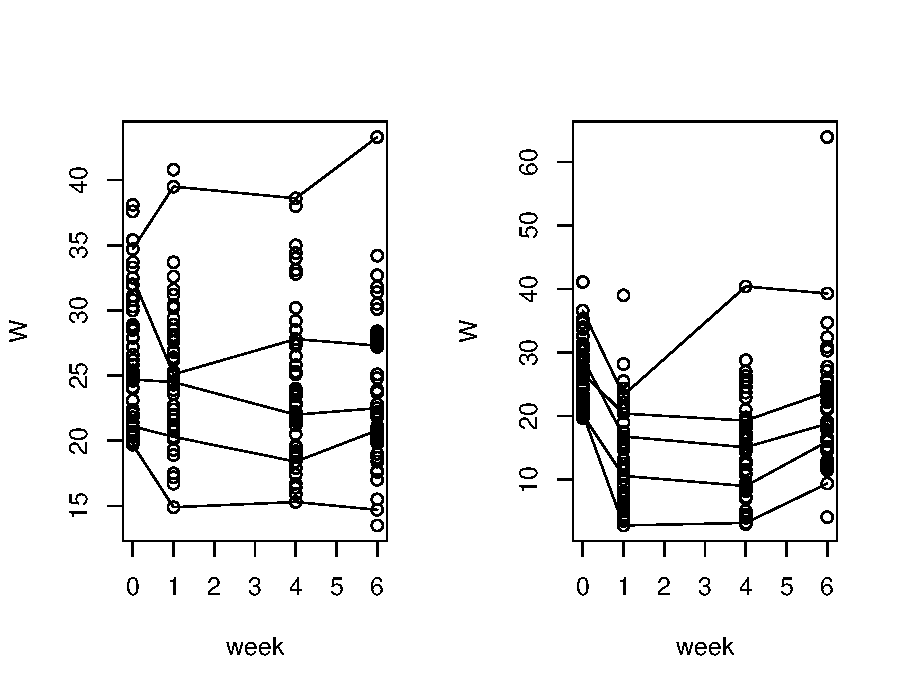
\includegraphics[width=\maxwidth]{figure/unnamed-chunk-3-4} 

}


\begin{kframe}\begin{alltt}
\hlcom{# This is a basic correlation plot It requires the}
\hlcom{# 'corrplot' library, which can be installed with}
\hlcom{# install.packages('corrplot')}
\hlstd{corrplot}\hlopt{::}\hlkwd{corrplot.mixed}\hlstd{(}\hlkwd{cor}\hlstd{(TLC_wide[}\hlkwd{c}\hlstd{(}\hlstr{"W0"}\hlstd{,} \hlstr{"W1"}\hlstd{,} \hlstr{"W4"}\hlstd{,} \hlstr{"W6"}\hlstd{)]),}
  \hlkwc{lower} \hlstd{=} \hlstr{"number"}\hlstd{,} \hlkwc{upper} \hlstd{=} \hlstr{"square"}\hlstd{)}
\end{alltt}
\end{kframe}

{\centering 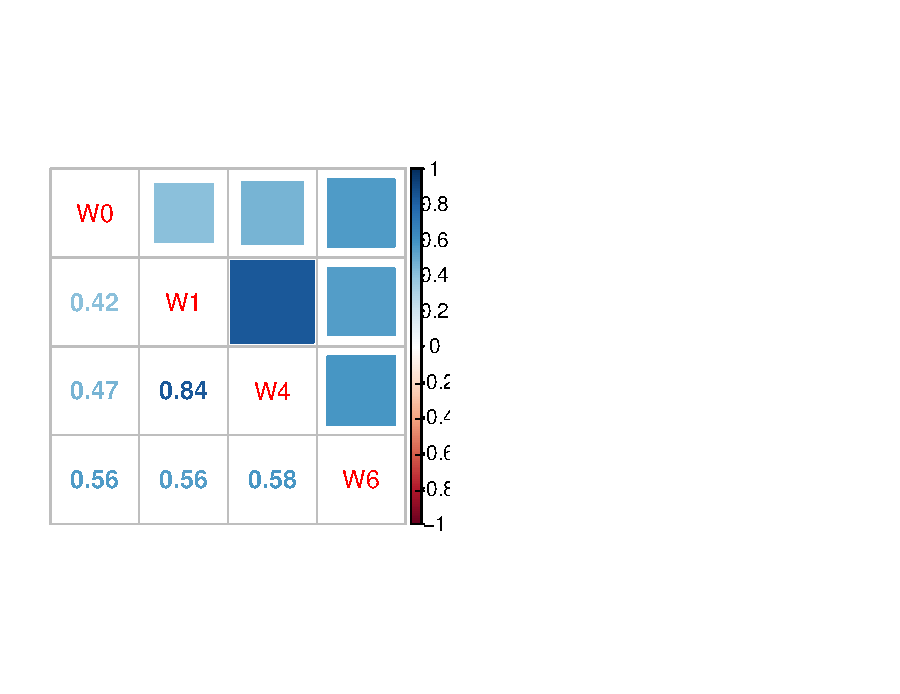
\includegraphics[width=\maxwidth]{figure/unnamed-chunk-3-5} 

}


\end{knitrout}
%\end{noindent}
\end{document}
